\documentclass{article}\usepackage[]{graphicx}\usepackage[]{color}
%% maxwidth is the original width if it is less than linewidth
%% otherwise use linewidth (to make sure the graphics do not exceed the margin)
\makeatletter
\def\maxwidth{ %
  \ifdim\Gin@nat@width>\linewidth
    \linewidth
  \else
    \Gin@nat@width
  \fi
}
\makeatother

\definecolor{fgcolor}{rgb}{0.345, 0.345, 0.345}
\newcommand{\hlnum}[1]{\textcolor[rgb]{0.686,0.059,0.569}{#1}}%
\newcommand{\hlstr}[1]{\textcolor[rgb]{0.192,0.494,0.8}{#1}}%
\newcommand{\hlcom}[1]{\textcolor[rgb]{0.678,0.584,0.686}{\textit{#1}}}%
\newcommand{\hlopt}[1]{\textcolor[rgb]{0,0,0}{#1}}%
\newcommand{\hlstd}[1]{\textcolor[rgb]{0.345,0.345,0.345}{#1}}%
\newcommand{\hlkwa}[1]{\textcolor[rgb]{0.161,0.373,0.58}{\textbf{#1}}}%
\newcommand{\hlkwb}[1]{\textcolor[rgb]{0.69,0.353,0.396}{#1}}%
\newcommand{\hlkwc}[1]{\textcolor[rgb]{0.333,0.667,0.333}{#1}}%
\newcommand{\hlkwd}[1]{\textcolor[rgb]{0.737,0.353,0.396}{\textbf{#1}}}%
\let\hlipl\hlkwb

\usepackage{framed}
\makeatletter
\newenvironment{kframe}{%
 \def\at@end@of@kframe{}%
 \ifinner\ifhmode%
  \def\at@end@of@kframe{\end{minipage}}%
  \begin{minipage}{\columnwidth}%
 \fi\fi%
 \def\FrameCommand##1{\hskip\@totalleftmargin \hskip-\fboxsep
 \colorbox{shadecolor}{##1}\hskip-\fboxsep
     % There is no \\@totalrightmargin, so:
     \hskip-\linewidth \hskip-\@totalleftmargin \hskip\columnwidth}%
 \MakeFramed {\advance\hsize-\width
   \@totalleftmargin\z@ \linewidth\hsize
   \@setminipage}}%
 {\par\unskip\endMakeFramed%
 \at@end@of@kframe}
\makeatother

\definecolor{shadecolor}{rgb}{.97, .97, .97}
\definecolor{messagecolor}{rgb}{0, 0, 0}
\definecolor{warningcolor}{rgb}{1, 0, 1}
\definecolor{errorcolor}{rgb}{1, 0, 0}
\newenvironment{knitrout}{}{} % an empty environment to be redefined in TeX

\usepackage{alltt}
\usepackage{Sweave}
\usepackage{float}
\usepackage{graphicx}
\usepackage{tabularx}
\usepackage{siunitx}
\usepackage{mdframed}
\usepackage{amsmath}
\usepackage{gensymb}
\usepackage{natbib}
\bibliographystyle{..//refs/styles/besjournals.bst}
\usepackage[small]{caption}
\setkeys{Gin}{width=0.8\textwidth}
\setlength{\captionmargin}{30pt}
\setlength{\abovecaptionskip}{0pt}
\setlength{\belowcaptionskip}{10pt}
\topmargin -1.5cm        
\oddsidemargin -0.04cm   
\evensidemargin -0.04cm
\textwidth 16.59cm
\textheight 21.94cm 
%\pagestyle{empty} %comment if want page numbers
\parskip 7.2pt
\renewcommand{\baselinestretch}{1.5}
\parindent 0pt

\newmdenv[
  topline=true,
  bottomline=true,
  skipabove=\topsep,
  skipbelow=\topsep
]{siderules}

%% R Script


\IfFileExists{upquote.sty}{\usepackage{upquote}}{}
\begin{document}

\renewcommand{\thetable}{\arabic{table}}
\renewcommand{\thefigure}{\arabic{figure}}
\renewcommand{\labelitemi}{$-$}
%%%%%%%%%%%%%%%%%%%%%%%%%%%%%%%%%%%%%%%%%%%%%%%%%%%%%%%%%%%%%%%%%%%%%%%%%%%%%%%%%%%%%%%%%%%
\section*{Chilling Experiment Figures}

\begin{figure} [H]
\begin{center}
\caption{Day of budburst and the day of leaf out for native tree species in New England. Data was collected from a growth chamber experiment using any combination of two photoperiod treatments, two forcing treatments, and three chilling treatments. The standard deviation is represented in blue for budburst and green for leaf out. }
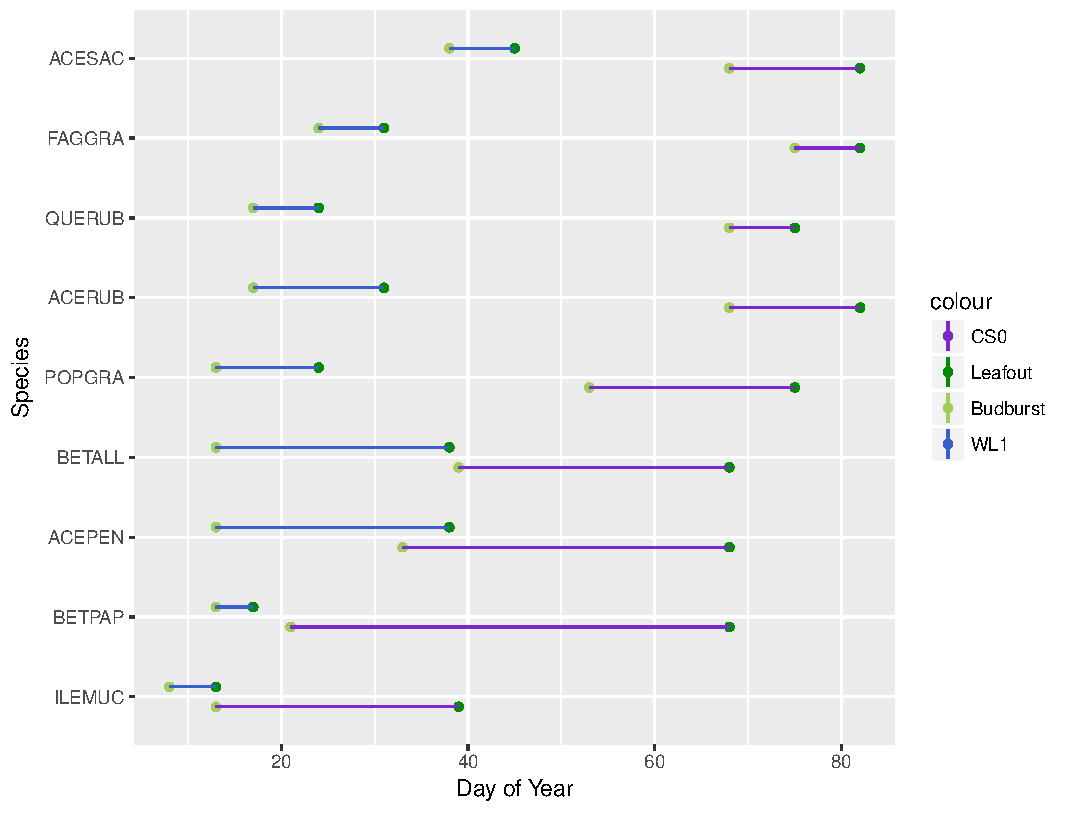
\includegraphics{..//figure/Exp_plot.pdf} 
\end{center}
\end{figure}


Anova Table (Type II tests)

Response: risk
          Sum Sq  Df  F value Pr(>F)    
chilling      32   1   0.3884 0.5333    
warm       14682   1 176.5185 <2e-16 ***
photo       6210   1  74.6629 <2e-16 ***
Residuals  82512 992                    
---
Signif. codes:  0 '***' 0.001 '**' 0.01 '*' 0.05 '.' 0.1 ' ' 1
Call:
   aov(formula = lm(risk ~ chilling + warm + photo, data = subby))

Terms:
                chilling     warm    photo Residuals
Sum of Squares   305.908 4209.929 1300.304  6684.850
Deg. of Freedom        1        1        1       108

Residual standard error: 7.867449
Estimated effects may be unbalanced
32 observations deleted due to missingness
Call:
   aov(formula = lm(risk ~ chilling + warm + photo, data = subby))

Terms:
                chilling     warm    photo Residuals
Sum of Squares     0.055 1616.346  462.883  6611.178
Deg. of Freedom        1        1        1       100

Residual standard error: 8.130915
Estimated effects may be unbalanced
28 observations deleted due to missingness
Call:
   aov(formula = lm(risk ~ chilling + warm + photo, data = subby))

Terms:
                chilling     warm    photo Residuals
Sum of Squares    63.855  184.380  224.826  4574.749
Deg. of Freedom        1        1        1        64

Residual standard error: 8.454611
Estimated effects may be unbalanced
76 observations deleted due to missingness
Call:
   aov(formula = lm(risk ~ chilling + warm + photo, data = subby))

Terms:
                chilling     warm    photo Residuals
Sum of Squares   241.871 1424.047  617.147  7183.300
Deg. of Freedom        1        1        1       133

Residual standard error: 7.349134
Estimated effects may be unbalanced
7 observations deleted due to missingness
Call:
   aov(formula = lm(risk ~ chilling + warm + photo, data = subby))

Terms:
                 chilling      warm     photo Residuals
Sum of Squares      1.299  1781.426  1104.063 10510.455
Deg. of Freedom         1         1         1       128

Residual standard error: 9.061618
Estimated effects may be unbalanced
12 observations deleted due to missingness
Call:
   aov(formula = lm(risk ~ chilling + warm + photo, data = subby))

Terms:
                 chilling      warm     photo Residuals
Sum of Squares    79.9153  734.1672    2.0829 2913.9060
Deg. of Freedom         1         1         1        66

Residual standard error: 6.644554
Estimated effects may be unbalanced
74 observations deleted due to missingness
Call:
   aov(formula = lm(risk ~ chilling + warm + photo, data = subby))

Terms:
                chilling     warm    photo Residuals
Sum of Squares    18.781 2261.937 1036.164  3334.911
Deg. of Freedom        1        1        1       136

Residual standard error: 4.951909
Estimated effects may be unbalanced
4 observations deleted due to missingness
Call:
   aov(formula = lm(risk ~ chilling + warm + photo, data = subby))

Terms:
                chilling     warm    photo Residuals
Sum of Squares    73.934 2219.117 1013.131  6777.906
Deg. of Freedom        1        1        1        98

Residual standard error: 8.316388
Estimated effects may be unbalanced
30 observations deleted due to missingness
Call:
   aov(formula = lm(risk ~ chilling + warm + photo, data = subby))

Terms:
                chilling     warm    photo Residuals
Sum of Squares    12.663  659.176  370.052  4972.536
Deg. of Freedom        1        1        1       127

Residual standard error: 6.257302
Estimated effects may be unbalanced
13 observations deleted due to missingness

% Error: Unrecognized object type.
% Error: Unrecognized object type.
% Error: Unrecognized object type.
% Error: Unrecognized object type.
% Error: Unrecognized object type.
% Error: Unrecognized object type.
% Error: Unrecognized object type.
% Error: Unrecognized object type.
% Error: Unrecognized object type.




\end{document}
